\section{Theoretical Framing}
\label{appendix:theory}

These are sufficient-condition results. They establish noise-odds and norm bounds under explicit assumptions; they do not establish distributional invariance or replace the empirical evidence.

\subsection{Extreme-value null floor}

\begin{assumption}[Sub-Gaussian noise scores]
For irrelevant keys $j\in\mathcal N_n$, $|\mathcal N_n|\leq n$, scores $X_j$ are mean-zero and $v^2$-sub-Gaussian: $\mathbb E\exp(tX_j)\leq\exp(v^2t^2/2)$ for all $t\in\mathbb R$.
\end{assumption}

Let the Polar null floor be $\nu_n=b+s\sqrt{\log(n+1)}$ with $b,s\geq0$.

\begin{proposition}[Noise exceedances]
Under Assumption 1,
\begin{equation}
\mathbb E\!\left[\sum_{j\in\mathcal N_n}{\bf1}\{X_j>\nu_n\}\right]
\leq n\exp\!\left(-\frac{\nu_n^2}{2v^2}\right).
\end{equation}
If $s\geq\sqrt2v$ this is $O(1)$; if the inequality is strict it decays polynomially.
\end{proposition}

\begin{proof}
Apply the sub-Gaussian tail bound to each key and sum. Since $b\geq0$, $\nu_n^2\geq s^2\log(n+1)$.
\end{proof}

Unlike TDA, Polar retains sub-threshold keys. With temperature $\theta_n=1+a\log n$, define the unnormalized noise-to-null odds $R_n=\sum_{j\in\mathcal N_n}\exp(\theta_n(X_j-\nu_n))$.

\begin{proposition}[Vanishing null odds]
Suppose $s>c>\sqrt2v$ and the null floor is $s\sqrt{\log(n+1)}$ up to a nonnegative offset. With probability tending to one,
\begin{equation}
R_n\leq n\exp\!\left(-(1+a\log n)(s-c)\sqrt{\log n}\right).
\end{equation}
For $a>0$, the bound converges to zero faster than any inverse polynomial.
\end{proposition}

\begin{proof}
A union bound gives $\Pr[\max_jX_j>c\sqrt{\log(n+1)}]\leq n(n+1)^{-c^2/(2v^2)}\to0$. On the complementary event, every noise score is at least $(s-c)\sqrt{\log n}$ below the floor. Bound each summand and sum over at most $n$ keys.
\end{proof}

\subsection{Bounded channels and recurrent state}

\begin{proposition}[Bounded Polar readout]
For $c_i=s_i/\max(\lVert s_i\rVert_2,\varepsilon)$, $\lVert c_i\rVert_2\leq1$. For $\mu_i=\tanh(\beta\log(1+m_{{\rm eff},i}))$, $\mu_i\in[0,1)$ when $\beta,m_{{\rm eff},i}\geq0$. A distribution uniform over $m$ real keys has participation ratio $m$.
\end{proposition}

\begin{proof}
The first two claims follow from the denominator and range of $\tanh$. Uniform weights satisfy $(\sum_{j=1}^m(1/m)^2)^{-1}=m$.
\end{proof}

\begin{assumption}[Contractive memory]
For every $t$, $\lVert q_t\rVert_2=\lVert k_t\rVert_2=1$, $\lVert v_t\rVert_2\leq V$, $0\leq\beta_t\leq1$, and $0\leq\gamma_t\leq\bar\gamma<1$.
\end{assumption}

\begin{proposition}[Length-bounded state]
For recurrence~\eqref{eq:memory},
\begin{equation}
\lVert M_t\rVert_F\leq\bar\gamma^t\lVert M_0\rVert_F+\frac{V}{1-\bar\gamma}.
\end{equation}
\end{proposition}

\begin{proof}
$I-\beta_tk_tk_t^\top$ has spectral norm at most one and $\lVert\beta_tv_tk_t^\top\rVert_F\leq V$. Thus $\lVert M_t\rVert_F\leq\bar\gamma\lVert M_{t-1}\rVert_F+V$; unrolling gives the result.
\end{proof}

The Lean artifact checks the finite-sum, exponential-monotonicity, bounded-channel composition, and invariant-set induction steps. It takes the sub-Gaussian tail, high-probability margin, and one-step contraction as premises. It is therefore a machine-checked proof skeleton, not end-to-end formal verification. The learned conditions $b\geq0$ and $s>c>\sqrt2v$ require an empirical head-wise audit before they can be asserted for a trained checkpoint.

\section{Evaluation Protocols}
\label{appendix:protocol}

Stage I contains 120 approximately 370--378M-parameter runs trained for 1,900 steps of 524,288 tokens at sequence length 2,048 on FineWeb-Edu. Stage II contains three matched attention models trained for 18,722 such steps (9.816B tokens). The five promoted checkpoints and ten open-weight controls are evaluated with checkpoint-exact forward paths.

Retrieval crosses passkey and NIAH tasks, synthetic and FinePDFs haystacks, eight lengths from 2K through 256K, three depths, and 50 paired trials per cell. The primary metric is teacher-forced accuracy over five target tokens. BABILong uses answer-only fine-tuning on tasks qa1--qa10 at 0K/1K/2K and greedy exact match on ten held-out rows per task and length. Base-task controls use LAMBADA, HellaSwag, PIQA, WinoGrande, ARC-Easy, ARC-Challenge, OpenBookQA, and BoolQ. Fixed-target BPB uses FinePDFs, PG-19, and Proof-Pile. All reported processes completed without failed, OOM, unsupported, missing, or null cells.

\section{Complete Factorial Sweep}
\label{appendix:full_ablation}

The complete 120-cell table is retained in the submission source and artifact. The main paper reports only the recipe transitions needed to justify promotion.
\begingroup
\fontsize{5}{6}\selectfont
\setlength{\tabcolsep}{1pt}
\begin{longtable}{llcccrccccc}
\caption{Complete Results of the 100-Run Ablation Sweep. All models are 370M parameters, trained on FineWeb-Edu for 1B tokens ($seq\_len=2048$). Evaluated from 2K to 64K context length. PPL is in nats (lower is better), Needle is accuracy in \% (higher is better), MFU is training model flops utilization in \%. \label{table:ablation_appendix}}\\
\toprule
Type & Reg & Dist & Mem & Win & Val Loss & PPL@2K & PPL@64K & Needle@2K & Needle@64K & MFU \\
\midrule
\endfirsthead
\caption[]{Complete Results of the 100-Run Ablation Sweep (continued).}\\
\toprule
Type & Reg & Dist & Mem & Win & Val Loss & PPL@2K & PPL@64K & Needle@2K & Needle@64K & MFU \\
\midrule
\endhead
\midrule
\multicolumn{11}{r}{{Continued on next page}} \\
\bottomrule
\endfoot
\bottomrule
\endlastfoot
POLAR & baseline & Off & Off & Off & 3.323 & 2.83 & 3.60 & 96.3 & 0.0 & 40.1 \\
POLAR & baseline & Off & Off & On & 3.343 & 2.83 & 2.66 & 67.5 & 0.0 & 39.6 \\
POLAR & baseline & Off & On & Off & 3.169 & 2.70 & 1.96 & 91.3 & 92.5 & 35.6 \\
POLAR & baseline & Off & On & On & 3.174 & 2.71 & 2.01 & 51.3 & 30.0 & 35.6 \\
POLAR & baseline & On & Off & Off & 3.332 & 2.81 & 5.56 & 85.0 & 0.0 & 33.3 \\
POLAR & baseline & On & Off & On & 3.361 & 2.85 & 2.89 & 91.3 & 2.5 & 34.5 \\
POLAR & baseline & On & On & Off & 3.178 & 2.72 & 1.98 & 73.8 & 58.8 & 31.8 \\
POLAR & baseline & On & On & On & 3.182 & 2.73 & 1.97 & 56.3 & 21.3 & 31.2 \\
POLAR & weak & Off & Off & Off & 3.333 & 2.82 & 2.86 & 88.8 & 0.0 & 39.0 \\
POLAR & weak & Off & Off & On & 3.348 & 2.90 & 3.76 & 93.8 & 0.0 & 37.9 \\
POLAR & weak & Off & On & Off & 3.179 & 2.74 & 1.95 & 70.0 & 51.3 & 36.2 \\
POLAR & weak & Off & On & On & 3.187 & 2.74 & 1.99 & 41.3 & 41.3 & 36.2 \\
POLAR & weak & On & Off & Off & 3.335 & 2.82 & 3.47 & 91.3 & 0.0 & 32.8 \\
POLAR & weak & On & Off & On & 3.353 & 2.82 & 2.58 & 96.3 & 1.3 & 32.8 \\
POLAR & weak & On & On & Off & 3.178 & 2.74 & 1.95 & 33.8 & 32.5 & 30.7 \\
POLAR & weak & On & On & On & 3.183 & 2.74 & 1.94 & 81.3 & 78.8 & 30.7 \\
POLAR & strong & Off & Off & Off & 3.338 & 2.85 & 3.79 & 98.8 & 1.3 & 37.3 \\
POLAR & strong & Off & Off & On & 3.360 & 2.85 & 2.99 & 91.3 & 0.0 & 37.9 \\
POLAR & strong & Off & On & Off & 3.172 & 2.72 & 1.96 & 80.0 & 52.5 & 35.8 \\
POLAR & strong & Off & On & On & 3.181 & 2.72 & 1.94 & 76.3 & 68.8 & 34.6 \\
POLAR & strong & On & Off & Off & 3.337 & 2.87 & 3.22 & 83.8 & 1.3 & 32.8 \\
POLAR & strong & On & Off & On & 3.347 & 2.82 & 2.64 & 97.5 & 16.3 & 32.2 \\
POLAR & strong & On & On & Off & 3.179 & 2.73 & 1.94 & 86.3 & 83.8 & 30.9 \\
POLAR & strong & On & On & On & 3.182 & 2.72 & 1.94 & 25.0 & 23.8 & 30.9 \\
POLAR & discrete & Off & Off & Off & 3.338 & 2.82 & 2.80 & 93.8 & 2.5 & 37.9 \\
POLAR & discrete & Off & Off & On & 3.349 & 2.87 & 2.90 & 93.8 & 6.3 & 37.9 \\
POLAR & discrete & Off & On & Off & 3.184 & 2.75 & 2.03 & 76.3 & 73.8 & 36.4 \\
POLAR & discrete & Off & On & On & 3.178 & 2.71 & 1.92 & 31.3 & 18.8 & 35.8 \\
POLAR & discrete & On & Off & Off & 3.333 & 2.80 & 4.13 & 97.5 & 0.0 & 32.6 \\
POLAR & discrete & On & Off & On & 3.351 & 2.87 & 2.72 & 85.0 & 2.5 & 33.3 \\
POLAR & discrete & On & On & Off & 3.189 & 2.74 & 1.96 & 87.5 & 53.8 & 31.8 \\
POLAR & discrete & On & On & On & 3.192 & 2.74 & 2.07 & 21.3 & 26.3 & 31.7 \\
POLAR & zipfian & Off & Off & Off & 3.338 & 2.85 & 4.83 & 96.3 & 11.3 & 37.9 \\
POLAR & zipfian & Off & Off & On & 3.350 & 2.83 & 2.58 & 88.8 & 3.8 & 39.4 \\
POLAR & zipfian & Off & On & Off & 3.171 & 2.70 & 1.92 & 52.5 & 63.8 & 36.2 \\
POLAR & zipfian & Off & On & On & 3.180 & 2.75 & 1.95 & 46.3 & 40.0 & 35.2 \\
POLAR & zipfian & On & Off & Off & 3.340 & 2.83 & 3.77 & 98.8 & 1.3 & 33.8 \\
POLAR & zipfian & On & Off & On & 3.352 & 2.85 & 3.13 & 90.0 & 0.0 & 33.5 \\
POLAR & zipfian & On & On & Off & 3.177 & 2.72 & 1.94 & 91.3 & 67.5 & 31.8 \\
POLAR & zipfian & On & On & On & 3.192 & 2.74 & 2.00 & 40.0 & 26.3 & 31.8 \\
NOPE & baseline & Off & Off & Off & 3.224 & 2.76 & 3.71 & 97.5 & 1.3 & 41.5 \\
NOPE & baseline & Off & Off & On & 3.219 & 2.75 & 2.76 & 92.5 & 10.0 & 36.5 \\
NOPE & baseline & Off & On & Off & 3.140 & 2.66 & 2.34 & 97.5 & 16.3 & 36.8 \\
NOPE & baseline & Off & On & On & 3.150 & 2.70 & 2.14 & 81.3 & 0.0 & 34.2 \\
NOPE & baseline & On & Off & Off & 3.209 & 2.74 & 2.99 & 90.0 & 18.8 & 32.5 \\
NOPE & baseline & On & Off & On & 3.212 & 2.77 & 2.90 & 81.3 & 0.0 & 30.3 \\
NOPE & baseline & On & On & Off & 3.149 & 2.67 & 2.35 & 80.0 & 16.3 & 30.0 \\
NOPE & baseline & On & On & On & 3.147 & 2.68 & 2.09 & 88.8 & 21.3 & 28.2 \\
NOPE & weak & Off & Off & Off & 3.214 & 2.77 & 3.10 & 95.0 & 0.0 & 40.9 \\
NOPE & weak & Off & Off & On & 3.222 & 2.75 & 3.05 & 81.3 & 0.0 & 36.1 \\
NOPE & weak & Off & On & Off & 3.147 & 2.68 & 2.07 & 88.8 & 21.3 & 37.5 \\
NOPE & weak & Off & On & On & 3.142 & 2.68 & 2.12 & 82.5 & 0.0 & 33.7 \\
NOPE & weak & On & Off & Off & 3.215 & 2.75 & 4.87 & 95.0 & 5.0 & 32.0 \\
NOPE & weak & On & Off & On & 3.221 & 2.73 & 2.63 & 81.3 & 0.0 & 29.3 \\
NOPE & weak & On & On & Off & 3.147 & 2.67 & 2.48 & 97.5 & 1.3 & 30.8 \\
NOPE & weak & On & On & On & 3.148 & 2.68 & 2.14 & 93.8 & 1.3 & 28.4 \\
NOPE & strong & Off & Off & Off & 3.231 & 2.74 & 4.88 & 90.0 & 2.5 & 38.4 \\
NOPE & strong & Off & Off & On & 3.214 & 2.72 & 2.68 & 82.5 & 0.0 & 36.4 \\
NOPE & strong & Off & On & Off & 3.144 & 2.68 & 2.37 & 96.3 & 6.3 & 35.7 \\
NOPE & strong & Off & On & On & 3.150 & 2.70 & 2.10 & 93.8 & 7.5 & 33.8 \\
NOPE & strong & On & Off & Off & 3.207 & 2.72 & 3.13 & 73.8 & 0.0 & 31.4 \\
NOPE & strong & On & Off & On & 3.214 & 2.74 & 2.49 & 86.3 & 8.8 & 28.9 \\
NOPE & strong & On & On & Off & 3.146 & 2.67 & 2.24 & 83.8 & 17.5 & 29.1 \\
NOPE & strong & On & On & On & 3.147 & 2.68 & 2.16 & 96.3 & 0.0 & 27.5 \\
NOPE & discrete & Off & Off & Off & 3.202 & 2.75 & 3.33 & 85.0 & 1.3 & 38.8 \\
NOPE & discrete & Off & Off & On & 3.234 & 2.79 & 3.11 & 70.0 & 18.8 & 37.0 \\
NOPE & discrete & Off & On & Off & 3.145 & 2.68 & 2.14 & 98.8 & 16.3 & 36.0 \\
NOPE & discrete & Off & On & On & 3.145 & 2.68 & 2.10 & 95.0 & 3.8 & 34.3 \\
NOPE & discrete & On & Off & Off & 3.212 & 2.88 & 3.04 & 42.5 & 0.0 & 31.2 \\
NOPE & discrete & On & Off & On & 3.211 & 2.78 & 2.73 & 82.5 & 1.3 & 29.1 \\
NOPE & discrete & On & On & Off & 3.145 & 2.68 & 2.27 & 91.3 & 11.3 & 30.3 \\
NOPE & discrete & On & On & On & 3.149 & 2.68 & 2.17 & 83.8 & 0.0 & 28.6 \\
NOPE & zipfian & Off & Off & Off & 3.209 & 2.71 & 3.18 & 90.0 & 0.0 & 40.8 \\
NOPE & zipfian & Off & Off & On & 3.219 & 2.75 & 2.71 & 77.5 & 1.3 & 36.1 \\
NOPE & zipfian & Off & On & Off & 3.141 & 2.67 & 2.55 & 96.3 & 0.0 & 38.0 \\
NOPE & zipfian & Off & On & On & 3.150 & 2.69 & 2.11 & 90.0 & 3.8 & 33.7 \\
NOPE & zipfian & On & Off & Off & 3.207 & 2.77 & 3.32 & 82.5 & 0.0 & 31.3 \\
NOPE & zipfian & On & Off & On & 3.227 & 2.79 & 2.91 & 93.8 & 11.3 & 30.2 \\
NOPE & zipfian & On & On & Off & 3.146 & 2.68 & 2.39 & 96.3 & 21.3 & 29.6 \\
NOPE & zipfian & On & On & On & 3.148 & 2.68 & 2.17 & 90.0 & 6.3 & 28.7 \\
ROPE & baseline & Off & Off & Off & 3.159 & 2.85 & 3.36 & 42.5 & 0.0 & 40.4 \\
ROPE & baseline & Off & Off & On & 3.163 & 2.86 & 3.79 & 15.0 & 0.0 & 37.2 \\
ROPE & baseline & Off & On & Off & 3.145 & 2.81 & 2.86 & 73.8 & 0.0 & 37.1 \\
ROPE & baseline & Off & On & On & 3.151 & 2.80 & 2.95 & 13.8 & 0.0 & 34.4 \\
ROPE & baseline & On & Off & Off & 3.163 & 3.00 & 3.47 & 38.8 & 0.0 & 33.2 \\
ROPE & baseline & On & Off & On & 3.167 & 2.88 & 4.06 & 0.0 & 0.0 & 30.2 \\
ROPE & baseline & On & On & Off & 3.153 & 2.73 & 2.45 & 75.0 & 0.0 & 31.4 \\
ROPE & baseline & On & On & On & 3.154 & 2.83 & 2.86 & 32.5 & 0.0 & 29.4 \\
ROPE & strong & Off & Off & Off & 3.165 & 2.78 & 3.34 & 30.0 & 0.0 & 39.0 \\
ROPE & strong & Off & On & Off & 3.158 & 2.85 & 2.63 & 51.3 & 0.0 & 35.9 \\
ROPE & strong & Off & On & On & 3.162 & 2.86 & 3.08 & 10.0 & 0.0 & 33.2 \\
ROPE & strong & On & Off & Off & 3.161 & 2.85 & 3.58 & 47.5 & 0.0 & 31.1 \\
ROPE & strong & On & On & On & 3.162 & 2.85 & 3.08 & 2.5 & 0.0 & 28.4 \\
ROPE & discrete & Off & Off & Off & 3.165 & 2.91 & 3.43 & 22.5 & 0.0 & 39.7 \\
ROPE & discrete & Off & Off & On & 3.158 & 2.84 & 4.05 & 3.8 & 0.0 & 36.9 \\
ROPE & discrete & Off & On & Off & 3.159 & 2.83 & 2.67 & 47.5 & 0.0 & 36.3 \\
ROPE & discrete & Off & On & On & 3.161 & 2.79 & 2.71 & 41.3 & 0.0 & 33.7 \\
ROPE & discrete & On & Off & On & 3.164 & 2.80 & 3.74 & 21.3 & 0.0 & 30.0 \\
ROPE & discrete & On & On & Off & 3.162 & 2.74 & 2.47 & 50.0 & 0.0 & 30.9 \\
ROPE & discrete & On & On & On & 3.154 & 2.79 & 2.68 & 18.8 & 0.0 & 28.9 \\
\end{longtable}

\endgroup

\section{Retrieval Breakdown}
\label{appendix:retrieval}

\begin{figure}[h]
\centering
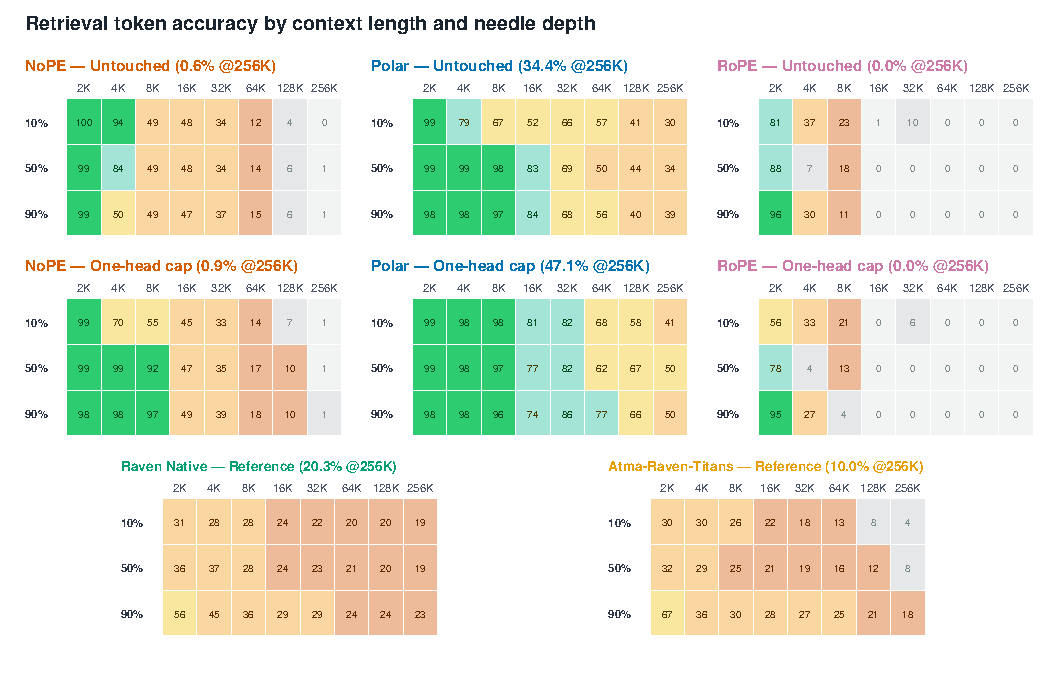
\includegraphics[width=\linewidth]{fig_niah_heatmap.pdf}
\caption{Retrieval depth sweeps for the five promoted models. Each cell is teacher-forced token accuracy.}
\end{figure}

\begin{table}[h]
\centering
\small
\resizebox{\linewidth}{!}{%
\begin{tabular}{llrrrrrrrr}
\toprule
\textbf{Model} & \textbf{Haystack} & \textbf{2K} & \textbf{4K} & \textbf{8K} & \textbf{16K} & \textbf{32K} & \textbf{64K} & \textbf{128K} & \textbf{256K} \\
\midrule
Polar & Synthetic & 99.6 & 98.4 & 98.5 & 97.0 & 94.9 & 92.3 & 80.3 & 68.4 \\
& FinePDFs & 98.6 & 86.3 & 77.9 & 49.1 & 40.7 & 16.3 & 3.2 & 0.3 \\
NoPE & Synthetic & 99.5 & 98.7 & 98.9 & 94.9 & 70.3 & 26.5 & 10.2 & 1.2 \\
& FinePDFs & 99.3 & 52.9 & 0.0 & 0.0 & 0.0 & 0.0 & 0.0 & 0.0 \\
RoPE & Synthetic & 81.7 & 44.9 & 33.1 & 0.8 & 6.8 & 0.1 & 0.0 & 0.0 \\
& FinePDFs & 94.8 & 4.7 & 0.2 & 0.0 & 0.0 & 0.0 & 0.0 & 0.0 \\
Atma-Raven-Titans & Synthetic & 64.8 & 60.7 & 51.1 & 46.9 & 41.7 & 35.8 & 25.9 & 19.3 \\
& FinePDFs & 23.2 & 2.6 & 0.7 & 0.2 & 1.4 & 0.5 & 1.6 & 0.7 \\
Raven Native & Synthetic & 55.9 & 57.7 & 51.4 & 48.3 & 44.3 & 40.9 & 38.9 & 35.1 \\
& FinePDFs & 22.1 & 15.4 & 8.2 & 3.3 & 5.3 & 2.9 & 3.7 & 5.4 \\
\bottomrule
\end{tabular}}
\caption{Zero-shot retrieval accuracy (\%) by haystack type and context length, averaged over needle depths.}
\end{table}

\section{Short-Context Quality and Systems}
\label{appendix:quality}

\begin{figure}[h]
\centering

\includegraphics[width=\linewidth]{fig_downstream_candle.pdf}
\caption{Eight short-context control tasks (22,939 examples per model).}
\end{figure}

\begin{figure}[h]
\centering

\includegraphics[width=\linewidth]{fig_serving_scaling.pdf}
\caption{Single-sequence serving on one L40S. Attention decode scales with KV-cache length; recurrent Raven uses fixed state.}
\end{figure}

\begin{table}[h]
\centering
\small
\resizebox{\linewidth}{!}{%
\begin{tabular}{llrrrrr}
\toprule
\textbf{Group} & \textbf{Model} & \textbf{Base mean} & \textbf{128K prefill} & \textbf{Decode} & \textbf{Peak alloc.} & \textbf{Train MFU} \\
& & (\%) & (s) & (ms/token) & (GiB) & (\%, 2K) \\
\midrule
Matched & NoPE & 45.1 & 1.47 & 16.4 & 39.40 & 42.77 \\
Matched & Polar & 43.3 & 1.62 & 16.3 & 39.41 & 40.44 \\
Matched & RoPE & 44.6 & 1.47 & 16.5 & 39.41 & 42.45 \\
Raven/AdamW & Atma-Raven-Titans & 43.1 & 1.00 & 2.27 & 8.62 & 30.92 \\
Raven/AdamW & Raven Native & 43.0 & 1.36 & 3.27 & 6.46 & 21.53 \\
\bottomrule
\end{tabular}}
\caption{Short-context quality and serving trade-offs. Serving uses one sequence and one timing sample; it is descriptive rather than an uncertainty estimate.}
\end{table}

\section{Stress and Environment Diagnostics}
\label{appendix:diagnostics}

\begin{figure}[h]
\centering
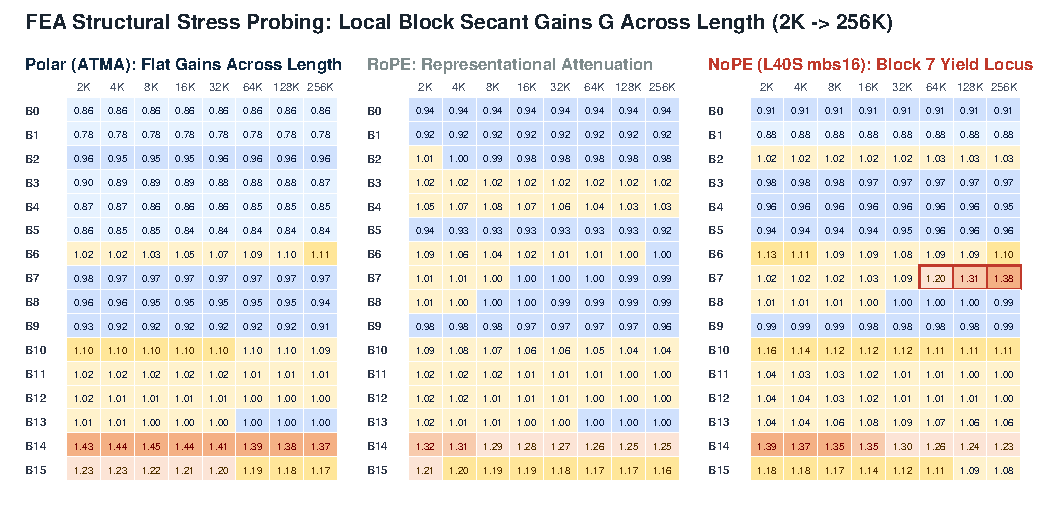
\includegraphics[width=\linewidth]{fig_stress_heatmap.pdf}
\caption{Block-wise sampled secant gains over 64 nested FinePDFs documents and 64 perturbation directions per document. The probe localizes checkpoint-specific changes but does not estimate a global Lipschitz constant.}
\end{figure}

For each block $f_i$, the diagnostic samples
\begin{equation}
G_i=\frac{\lVert f_i(x+\delta x)-f_i(x)\rVert_{\rm rms}}{\lVert\delta x\rVert_{\rm rms}},
\qquad \lVert\delta x\rVert_{\rm rms}=0.02\lVert x\rVert_{\rm rms}.
\end{equation}
The maximum sampled gain is a lower bound on the local operator norm along sampled directions; it is not a tight bound on the block Lipschitz constant. In the observed NoPE collapse, changes first concentrate near blocks 6--7 and later propagate through the residual stream. Polar's sampled gains and activation moments remain comparatively flat through 256K.

The environment diagnostic re-evaluates checkpoints under PyTorch 2.12 and 2.13, compares microbatch 4 and 16 on L40S, and uses deterministic short-context stream fixtures. These controls rule out evaluation-version and microbatch-only explanations in the tested runs. They do not isolate a unique low-level cause, because the L4/L40S intervention was not replicated over multiple training seeds and kernel configurations.
